\scanpage{92}
\mspage{88}
% archive sheet number: 91

\[
\underbrace{\operatorname{supp}^{\circ}_E(A)}_{\bar A}\mid\circ\mid\operatorname{supp}^{\circ}_E(\bar\beta(A')\ \Longleftrightarrow\ \operatorname{supp}^{\circ}_{E'}(\bar\alpha(A))\mid\circ\mid\underbrace{\unsure{\operatorname{supp}^{\circ}A'}}_{\bar A'}
\tag*{(*)}
\]
\deleted{Si on \unsure{prouve} qu'on a}
\[
\deleted{\operatorname{supp}^{\circ}_E(\bar\beta(A'))=\operatorname{supp}^{\circ}_E}
\]
\deleted{\unsure{Si on pouvait}}\inserted{Or dans (iii) b)} On a supposé
\[
\left\{
\begin{aligned}
\operatorname{supp}^{\circ}_E(\bar\beta(A'))&=\operatorname{supp}^{\circ}_E(\bar\beta(\bar A'))\ \bigl(\overset{\text{\unsure{def|déf}}}=\beta_{\unsure{*|\ell}}(\bar A')\bigr)\\
\operatorname{supp}^{\circ}_{E'}(\bar\alpha(A))&=\operatorname{supp}^{\circ}_{E'}(\bar\alpha(\bar A))\ \bigl(\overset{\text{def}}=\alpha_*(\bar A)\bigr)
\end{aligned}
\right.
\tag*{(**)}
\]
on en conclut que (*) s'écrit aussi
\[
\bar A\mid\circ\mid\beta_*(\bar A')\ \Longleftrightarrow\ \alpha_*(\bar A)\mid\circ\mid\bar A'
\]
ce qui n'est autre que (iii).
\figure{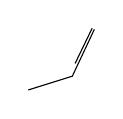
\begin{tikzpicture}[x=0.7cm,y=0.7cm]
\draw (0,0)--(0.8,0.25)--(1.2,1.1);
\draw (0.85,0.48)--(1.16,1.12);
\end{tikzpicture}}
Donc il \deleted{faut}\inserted{reste à} prouver \inserted{que (ii) \unsure{implique},} les deux relations (**) -- et il suffira \deleted{\unsure{de pr}} (par raison de symétrie) de prouver la seconde :

\uline{Corollaire 1} Sous les conditions du lemme 1 (en l'occurrence, sous la forme (ii)), si $A\in\unsure{\mathscr{P}|\mathcal{P}}(E)$, $A'\in\mathscr{P}(E')$, $\bar A=\operatorname{supp}^{\circ}_E(A)$, $\bar A'=\operatorname{supp}^{\circ}_{E'}(A')$, on a les relations (**) ci-dessus.

\uline{Dém} Comme $A\subset\bar A$, on a $\bar\alpha(A)\subset\bar\alpha(\bar A)$ d'où $\operatorname{supp}^{\circ}_{E'}(\bar\alpha(A))\subset\operatorname{supp}^{\circ}_{E'}(\bar\alpha(\bar A))$, il faut prouver $\unsure{\supset|\supseteq}$. Il revient au $=$ de dire que $\forall A'\in\Sigma_{E'}$, on a
\[
A'\mid\circ\mid\deleted{\operatorname{supp}^{\circ}_{E'}}(\bar\alpha(A))\ \Longleftrightarrow\ A'\mid\circ\mid\deleted{\unsure{\operatorname{supp}^{\circ}_{E'}}}\deleted{\unsure{\alpha_*(\bar A)}}(\bar\alpha(\bar A))
\]
